\chapter{Stashing Your Cash}
\fancyhead[CO]{\emph{Stashing Your Cash}}
\fancyhead[CE]{Freedom Beckons}

As you earn more and spend less, your money will start accumulating. You will need to put it somewhere. This is the third piece of financial independence: investing. How you invest your money is very important because it will eventually become your entire or partial source of income. As your savings accumulate, it's important to have a sound investment strategy. It may not seem quite so important at the beginning, but the magic element of investment growth is time, so the choices you make early on will be magnified over time.

The best investment strategies require very little maintenance. People who invest in something solid and leave it there tend to do better than those who move their money around a lot. So, once you find an investment strategy you feel comfortable with, you'll essentially be done. The rest is just investing according to that strategy. Do this early, and then you can focus on the rest.

The basics of investing are fairly straightforward and can be used by most people to develop a decent set of investments. Like many subjects, it does have a lot of depth, but it's up to you how deep you'd like to go. The deeper you go, the more efficient and effective your investments will be, so it's worth the effort. You can still achieve financial independence with less effort, but it will likely take you longer. This is another trade-off you must consider for yourself.

This book is based on the assumption that you are willing to do a lot of your own research and put a lot of effort into finding the most effective way for you to earn, save, and invest your money. Therefore, I go into investing in some depth in this book, but this is still just scratching the surface. There are some books I highly recommend for you to complete your investment training. Nonetheless, even in this book, I try to make it easy for you to choose for yourself how deep you want to go. I will present some easy and increasingly complex investment strategies, and let you decide.

\section{Disclaimers}
Investing isn't brain surgery, but it does share one thing with it: practiced incorrectly, it can be disastrous to your health---your financial health. While what I present here is time-tested and recommended by many of the leading investors and academic economists, I am not a certified financial planner. I'm just someone who has studied this extensively and has been able to use this knowledge to retire at an early age.

If you choose to do your own investing, which I recommend, you're taking the risk of misunderstanding something you read, not noticing or not taking warnings seriously when you read them, or otherwise incorrectly executing what you learn.

On the other hand, if you don't do your own investing, you're taking the risk that your financial planner is incompetent, doesn't have your best interests at heart, or both. Unlike brain surgeons, who risk malpractice lawsuits, financial planners are more likely to take advantage of their clients. The legal regulation of the financial planning industry is paltry compared to brain surgery. It's up to you to decide whether it's worth the risk to trust a financial planner.

There are several other risks you face by investing, and it's impossible to eliminate them all. Even if you invest in only government bonds, assumed to be the safest investment around, you face \emph{inflation risk,} which is the risk that the money you've invested will be able to buy less in the future, and \emph{interest rate risk,} which is the risk that the interest rates will change. Most intelligent investors believe the inflation risk of government bonds alone are worse than any of the other risks. These include, but are not limited to, \emph{currency risk,} which is the risk that the value of the currency your investments are held in will change by switching to a different currency; \emph{liquidity risk,} which is the risk that you won't be able to cash out; \emph{financial risk,} which is the risk that companies or governments will face some internal disruption; \emph{market risk,} which is the risk that supply and demand will significantly affect your investments; and \emph{credit risk,} which is the risk that loans won't be paid off.

In other words, it's possible you're going to ``lose your shirt,'' ``take a bath,'' or whichever clich\'e you prefer for ``lose way more money than you ever dreamed possible.'' This can be scary for some people, and thrilling for others. It might keep you up at night. The risks are there, and you should know about them, so you can invest with your eyes open. The whole point of this book is awareness of trade-offs, and risk is one of the factors you must consider when you weigh your trade-offs. One of the cardinal rules of investing is the trade-off between risk and return: greater risks are usually compensated with greater returns and safer investments tend to have a lower return.

There are many ways to manage risk, which I will discuss at length. You should know your own \emph{risk tolerance,} which is how emotional you get when your investments go up and down. If you know your risk tolerance when you go in and invest accordingly, it shouldn't be too scary. It only gets scary when you get in over your head, taking on more risk than you can handle. For this reason, I recommend that you start out conservatively if you're not experienced with investing. You should assume you have a lower risk tolerance than you think. After some experience, you can adjust it. Or you may decide that those risks really are worth the reward. That's your choice.

Despite all the risks, it's still better to invest than not. It's impossible to avoid investment risks, even if you avoid investing entirely. You still have \emph{job risk,} which is the risk that the company you work for invests poorly and lays you off; \emph{economic risk,} which is the risk that the economy as a whole plunges, leaving you out of work entirely; and the biggest risk of all: \emph{opportunity risk,} which is the risk that you will miss out on investment opportunities. More money is lost from opportunity risk than all the other risks combined.

\section{Investing basics}
Like spending, investing is also very personal. Your investment strategy will depend on a number of factors specific to you. One is your \emph{age.} A related concept is \emph{time horizon,} the amount of time between now and when you plan to liquidate your investments. The younger you are or the farther out your goal is, the longer you have to weather volatility in your investments. If you can weather short-term risk then you can gain higher long-term returns. Another is your goal. In the case of this book, I will assume your goal is financial independence. Another is your risk tolerance. All three factors should be measured and accounted for in your investment strategy.

There are many different \emph{investment vehicles,} or places to put your money, that will give you some interest or return. The most important investment vehicles are stocks and bonds.

A \emph{stock} is a small piece of ownership of a company or asset, like real estate or precious metals. You literally own part of the company, or a share of assets, and you get paid a chunk of its earnings, which are called \emph{dividends.} You may also sell stocks on the open market, and how much you can buy or sell it for can vary drastically over time. Any gain you get from selling a stock for more than you bought it is called a \emph{capital gain.} Stocks are the most powerful investment vehicle around for long-term investing because they provide the greatest long-term return, although they also involve quite a bit of short-term risk.

A \emph{bond} is a share of a loan. Organizations, usually governments or businesses, need loans for temporary costs, much like a homeowner would take out a loan for an improvement on their house. However, these institutions need much larger loans than homeowners do, so they divide it up into many smaller loans, called bonds. These bonds have an interest rate, sometimes called the \emph{coupon,} which is a certain percentage that the bond seller promises to pay you in addition to paying back the loan. Like stocks, you can buy and sell bonds on the open market, so in addition to the interest, you can also get a capital gain from bonds. There are also \emph{zero-coupon bonds.} These don't pay interest but are sold at a \emph{discount} from their \emph{face value,} which it will be worth on its \emph{maturity date.} Basically, you buy these bonds for a certain price, and the organization promises to pay you back a higher amount at a certain date.

A \emph{mutual fund,} or just \emph{fund,} is an aggregation of many stocks, many bonds, or both together. This is the most common way to invest because it's the easiest and cheapest way to diversify, which I will explain shortly.

Here are some other investment vehicles you should know about:
\begin{itemize}
\item \textbf{Savings account} --- An account at a bank that pays interest, which has minor limitations on how often or how easily you can withdraw money. The ease with which you can withdraw money is called \emph{liquidity.} Savings accounts are very liquid, but not as liquid as checking accounts.

\item \textbf{Money market fund} --- This is like a savings account, but it offers limited check writing capabilities, and it used to offer better rates than savings accounts, but now they offer roughly the same rates. Traditionally, money market funds weren't covered by \emph{FDIC insurance,} a government guarantee in case the bank goes under, so they had more risk than savings accounts, but that changed in 2008. Nowadays, you can treat money market funds like savings accounts that sometimes offer a limited check writing feature.

\item \textbf{CD, or Certificate of Deposit} --- This has a date, called the \emph{maturity date}, that you must wait until before you can withdraw money. This can be anywhere from one month to several years. Having to wait to withdraw obviously means it's not as liquid as a savings account, and in exchange for promising to wait, you're supposed to be rewarded with a higher rate of return. I usually find this reward to be small or non-existent compared to money market funds and savings accounts, so I don't bother with CDs.
\end{itemize}

\section{Schools of thought}
There are many different schools of thought and points of debate in investing, particularly in stocks. One debate is over \emph{long-term investing} versus \emph{day trading.} Long-term investors believe that the best strategy is to buy good investments and keep them as long as possible, while day traders time their investments so they can buy low and sell high. The traders themselves debate between \emph{fundamental analysis} and \emph{technical analysis.} Fundamental analysis focuses on the fundamental aspects of a company, such as how much money they have and how much they earn. Technical analysts simply look at past trends of stock prices and project those trends into the future.

Another point of debate is over \emph{value investing} versus \emph{growth investing.} Value investors look for good companies that are going through tough times, so they can buy them at low prices, kind of like looking for sales at your supermarket. Growth investors look for good companies that are very successful and seem poised for future growth, and are less concerned about their cost.

Although I described these as debates between polar opposites, reality is more complex. Many investors think long-term, but are also keen about timing their trades. Fundamental analysis and technical analysis are often used in conjunction. Many value investors believe their stocks are also good stocks that are poised for growth, and the only difference is in whether price matters. A lot of investors have some value stocks as well as some growth stocks. In fact, this is a wonderful strategy for \emph{diversification,} which is yet another debate.

Diversification can also be called \emph{asset allocation.} It means owning several different kinds of investment vehicles, and stocks in particular, that tend to behave in different ways. It's argued that this will provide a greater return with less volatility and less risk. Others believe that owning so many stocks means owning a lot of dead stocks, which dilutes the returns. They argue that you need no more than 15 different stocks to sufficiently manage risk, so if you can pick 15 really good companies, you'll do better than if you have hundreds or thousands. But asset allocators argue that it's impossible to predict which companies will be successful, and that most people tend to get better returns by aiming for the average than by trying to pick the right stocks. This is called the \emph{random walk theory.}

A more recent debate is over \emph{socially responsible investing, or SRI.} This is investing with your conscience, only owning companies that have a record of treating employees, communities, and the environment ethically. SRI investors argue that, in addition to being better ethical choices, these companies also perform better over the long run because they have happier customers, happier employees, and fewer lawsuits. This is a relatively new twist in investing, so it's hard to tell how well it actually works in practice, over the long run. The biggest known disadvantage of SRI funds is that they tend to cost a lot more than non-SRI funds. Maybe the only real advantage of SRI funds is that investors feel better about the ethical aspect of their investments. This may be intangible, but is very important to some investors.

I've toyed with every approach to investing and trading I've talked about. They each have their pros and cons. You'll hear a lot about all of them if you pay attention to the investing media. But I knew I needed to converge on a strategy for my own needs, and for that, I decided to mostly ignore the media, which seemed to be all over the board. The media, I realized, has no incentive to measure and quantify the effectiveness of each of these strategies, and report on their findings. The media's goal is to have a lot of readers and viewers. For that, they need excitement, and what is more exciting than a lively debate? They also emphasize day trading over long-term investing because day trading is a lot more exciting. Long-term investing is about as exciting as watching plants grow.

I decided to focus my attention on the experts, those who aren't trying to stir up debate, entertain audiences, or sell their own products, but are only trying to find which strategies have proven to be the best. These are the academic economists and the most successful private investors. When I focused on these experts, I found very little debate. They were mostly in agreement and recommended the same strategy for amateur investors, based on \emph{Modern Portfolio Theory,} which I will explain later in this chapter.

\section{The problem with bonds}
One approach to investing is to eschew stocks altogether, and only own bonds. The extreme form of this is to only buy treasury bonds. This does have certain advantages. It has the least volatility and least risk of losing money. Its low volatility means that you don't need to mess around with withdrawal rates (which I mentioned briefly in the last chapter, and will talk more about in Chapter 5) because you can just spend what the bonds pay. However, this strategy has two fatal flaws: \emph{interest rate risk} and \emph{inflation risk.}

Because these bonds are so safe, they also have a very low return. This return can vary over time, and the government has been known to bring the interest rates down to zero. This ability to drastically change interest rates is an important tool the government uses to ease the ebbs and flows of the economy. Even if you score some bonds that pay high interest, it's impossible to know how the rates will change in the future.

Much of the time, bond interest rates are less than \emph{inflation,} the tendency for costs to rise over time. This means you'll not only not earn enough to accomodate financial independence, but you'll effectively be losing money. There is some debate as to how to measure inflation, and how realistic those measurements actually are for the average consumer. It can be tempting to overlook inflation, especially if you're frugal. If you're not buying much of those big expensive items that inflation measures tend to focus on, then maybe you don't need to worry about inflation at all.

However, inflation is still a very real risk, even if you're frugal. After all, you still have to spend your money on something. Food prices go up, land values rise, and health costs go through the roof. Inflation is impossible to predict. It might not affect you much, or it might hit you very hard.

I figured, it's better to plan for inflation and be wrong than ignore inflation and be wrong. However, I wasn't paranoid about it either. I planned for a modest level of inflation. Assuming a very high inflation rate carries with it the risk of delaying my financial independence unnecessarily.

So far, inflation hasn't really impacted my retirement. My capacity to continually cut costs has outpaced inflation. Some specific expenses are definitely higher, such as gas and health care, but most of my other expenses have dropped. My overall expenses are higher than they were when I retired, but that's because my boss gave me raises (even though I'm retired, I still feel like I have a boss, and he gives me raises. See Chapter 5).

There is only one investment vehicle that is practically guaranteed to out-pace inflation: stocks. The reason is that inflationary price increases are made by companies, which means more income, which means more dividends and capital gains for investors. Most companies grow in many ways other than inflating prices, so they are able to out-pace inflation. For the sake of diversification, you should have some bonds in addition to stocks, but the majority of your investments should probably be in stocks.

There is a new form of U.S. Treasury Bond that is specifically designed to beat inflation. It's called \emph{TIPS,} which stands for \emph{Treasury Inflation-Protected Securities.} They take last year's inflation rate, measured by a standard index, and then pay some rate on top of that. This is a tool for managing inflation risk in Treasury bonds. If you only want to invest in bonds and live on the interest, I'd recommend using TIPS. However, this still doesn't manage the \emph{opportunity risk} or \emph{interest rate risk.}

Since there are ways to manage the risks of investing in stocks and corporate bonds, I believe these are the best investments for financial independence.

\section{Investing made easy}
Learning about investing makes a lot of people's eyes glaze over. In this chapter I briefly explained all the absolute basics of investing, without much detail. Check the Resources section if you would like to learn more. What I'm going to do next is explain the investment strategy I recommend for financial independence, how that strategy works, and why. That will involve a certain amount of detail, and although I will try to keep it as easy as possible, learning the details about investing necessarily means lots of numbers, \% and \$ signs, and new jargon that I will be introducing along the way.

Here are two easy investment choices to get us started.

The easiest approach is probably to \textbf{buy a pre-packaged portfolio} called a \emph{balanced fund.} This is almost as easy as opening a savings account at a bank. You just buy one fund and that's it. They take care of the allocations and rebalancing. All you need to do is contact the fund provider and ask for the fund. They will ask you a few basic questions about your goals, and then you send them your deposits. You can also do this online. Balanced funds are easy and cheap, but they are fairly generic, not very customized to your needs, so they won't provide the optimal performance and risk management for your goals.

The easiest way to create a portfolio customized to your exact needs is to \textbf{hire a financial planner.} They'll interview you, ask you questions about your financial situation and goals, and come up with a plan that works for you. They will describe it in simple terms, and if you feel comfortable with it, you'll write them a check, and you're good to go. They'll continue to work with you, so if you ever have questions or concerns about your investments as the economic weather changes, you can call them up. They'll keep you from doing deadly things like buying into the latest fad or selling everything when you get scared.

However, planners are \emph{very} expensive, and these costs come straight out of your investment growth. Few investors fully appreciate just how much these costs hurt their investments over time, and many planners are loathe to make this very clear. They may argue that their returns are so fabulous that your costs will be covered many times over, but research into this industry does not bear this out. Due to their high costs, they have to vastly outperform the overall market just to break even. Most financial planners merely match the returns of the market as a whole, and many even under-perform the market, so the costs do matter a great deal.

To make matters worse, there is a lot of incompetence in this field. Most planners are trained more in sales than in investing, and their certification process isn't very sophisticated. Make sure you get a referral from a trusted source, and interview the planner thoroughly. Ask to see how their other portfolios have done, ask how their fee structure works, and shop around. To fully appreciate the impact their costs will have, ask for a comparison between how much money you could reasonably expect to have in several decades without costs versus with their costs. Make sure they understand and support your financial independence goals. Some will tell you it's not possible, but that just means they don't know how.

Hiring a financial planner is theoretically easy, but the minefield of high costs and bad planners definitely sours it. In the Resources, I provide URLs for balanced funds and financial planners I recommend, both from Vanguard. I'm very distrusting of the investment industry in general, but Vanguard has been a breath of fresh air for me. I have found that they consistently offer the lowest fees and the best customer service.

If you'd rather take total control over your own investments, and you're ready to venture into the wild and exciting world of investing, then read on!

\section{Modern Portfolio Theory}
The investing strategy I recommend is buying and holding a well-diversified portfolio of low cost index funds of stocks and bonds, employing Modern Portfolio Theory.

\emph{Index funds} are mutual funds that just buy and hold shares that track a market index. An index represents some segment of the stock or bond markets. It's essentially just a list of companies. The index rarely changes, so the fund also rarely trades. The index represents the average return of these markets, but since taxes and fees are much lower, you can expect above-average returns from them. Index funds may sound mediocre or even drab, but they're actually very powerful in their simplicity.

Despite their enormous fees, most mutual funds usually \emph{under-perform} the indexes, often with \emph{more risk.} The impact of management fees in mutual funds is not immediately obvious. Because the fee rates are subtracted from the return rates rather than multiplied, a tiny difference in fees can mean an enormous difference in returns.

For example, let's say a fund returns 5\% in a particular year, a decent but unremarkable return, and it charges 1\% in management fees. This 1\% is \emph{subtracted} from the return rate, not multiplied. Your 5\% return becomes 4\%, not 4.95\%. In other words, you didn't lose 1\% of your return but 20\%! This is a big hurdle for a fund to overcome. The management has to add an enormous amount of value, just to pay for itself. Few pull it off.

Regular mutual funds tend to charge between 0.50\% to 2.00\%. Index funds are not actively managed, so their fees tend to be between 0.10\% and 0.20\%. Using the same example with a 0.15\% management fee, now you're only losing 3\% of your return. Index funds are also more tax-efficient than most mutual funds because there's much less turnover, creating less capital gains taxes.

When you account for the huge overhead of fees and taxes, index funds almost always out-peform most funds. It is \emph{possible} to find that rare fund that can out-perform index funds, but it's impossible to know ahead of time which funds those will be. Most of yesterday's stars are tomorrow's dogs.

\emph{Modern Portfolio Theory (or MPT)} is an investment theory that seeks to maximize investment returns while minimizing risk. It may seem almost magical when you first see it in action, but it's very real, and very powerful. A good way to describe MPT is ``the whole is greater than the sum of its parts.'' A good analogy is sodium chloride. Separately, sodium and chloride are explosive chemicals, but put them together and you get table salt. It sounds magical, but it's really quite natural. That's kind of how MPT works.

Modern Portfolio Theory is based on diversification and \emph{asset allocation.} The goal is to get lots of these different kinds of investment vehicles, or \emph{asset classes,} together in a \emph{portfolio,} which is just a conceptual grouping of all your investments.

For example, if you have \$10,000 to invest, you might put \$2,000 in bonds, \$2,000 in growth stocks, \$3,000 in value stocks, and \$3,000 in international stocks. That's a diversified portfolio of investments. Its asset allocation is 20\% in bonds, 20\% in growth stocks, 30\% in value stocks, and 30\% in international stocks. In each of these categories, you'd tend to own one or more funds, each of which may have hundreds or even thousands of individual stocks or bonds. What you end up with is a collection of funds, called a \emph{portfolio.}

Before MPT, investors didn't think much about their portfolio as a whole. It was just a collection of individual investments, and they focused on how each of these performed separately. MPT showed that the behavior of each of the parts plays off of each other to have different effects on the portfolio as a whole. The portfolio, if arranged properly, can have a higher return and lower volatility than any of the funds contained therein.

Let's illustrate how this works. Suppose you have \$10,000 to invest, and you decide to invest it in one of two funds that are known to be volatile but give excellent returns over time (it's generally understood that the more volatile a fund, the higher its return over time).

You buy \textbf{Fund A} for \$10 per share. The next year it's worth \$9 per share, the next year it's \$8 per share, and the next year it's \$12 per share. It's up 20\% after three years, but it was on quite the joy ride along the way. Had you invested in only this fund, then after three years, your \$10,000 would now be \$12,000. That would feel pretty good, but you weren't feeling so hot last year when it had shrunk to \$8,000.

Suppose instead you bought \textbf{Fund B}, also for \$10 per share. Next year it's worth \$11, the year after it's \$13, and the year after that it's \$12. Had you invested in only this fund, then after three years, your \$10,000 would now be \$12,000. Also very good, but you're probably kicking yourself for not selling it last year when it was worth \$13,000.

Now let's suppose you used MPT and allocated your money \textbf{50/50 between both funds.} Instead of \$10,000 in one fund, you invest \$5,000 in each of two funds. At some point, you \emph{rebalance,} which means buying and selling the funds in order to bring your allocation back to half and half. Let's see how you would have done.

You buy 500 shares of Fund A at \$10 per share and 500 shares of Fund B at \$10 per share, which is \$5,000 in each, for a total of \$10,000. In the second year, your portfolio would still be worth \$10,000. Already, the volatility is down. Although each fund is quite volatile separately, together your portfolio as a whole hasn't budged. The losses from one was offset by the gains in the other.

To rebalance, you calculate the new percentage of each fund in your portfolio. Fund A has 500 shares, now worth \$9 per share, which is \$4,500. Fund A has 500 share, now worth \$11 per share, which is \$5,500. Fund A is 45\% and Fund B is 55\%. You sell \$500 of Fund B and buy \$500 of Fund A. You should now have about 556 shares of Fund A and 455 shares of Fund B.

In the third year, your portfolio would be worth \$10,363. Notice how smooth your growth has become? Your individual funds are going crazy, but your portfolio as a whole is seeing a slow and steady progression upwards. After rebalancing again, you have about 648 shares of Fund A and 399 shares of Fund B.

By the end, your portfolio would be worth \$12,564. This is slightly better than you could have done with either fund individually. What we have here is a technique that gives you the best of both worlds: less volatility \emph{and} better performance.

\begin{figure}
\centering
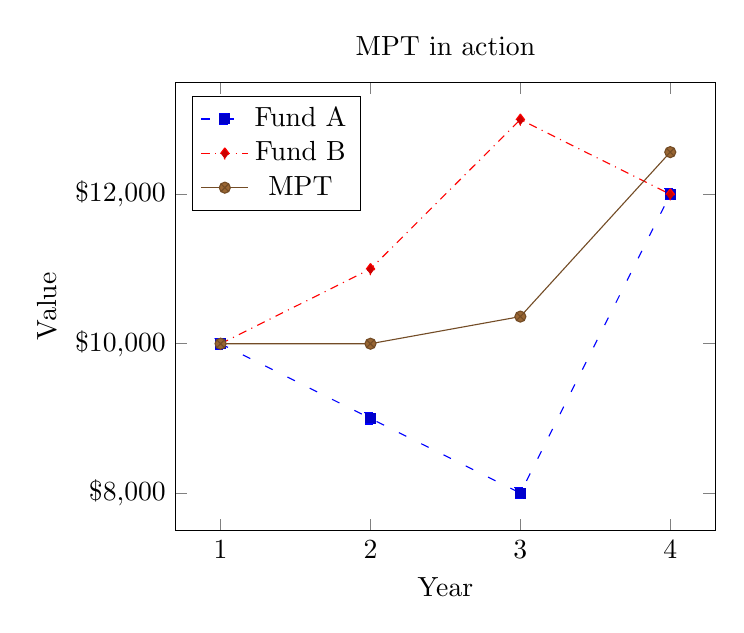
\begin{tikzpicture}
\begin{axis}[
    title=MPT in action,
    xlabel={Year},
    ylabel={Value},
    xtick={1,...,4},
    scaled y ticks=false,
    legend pos=north west,
    yticklabel={$\$\pgfmathprintnumber{\tick}$},
]
\addplot+[
    style={loosely dashed},
    mark={square*},
] coordinates {
    (1, 10000)
    (2, 9000)
    (3, 8000)
    (4, 12000)
};
\addplot+[
    style={dashdotted},
    mark={diamond*},
] coordinates {
    (1, 10000)
    (2, 11000)
    (3, 13000)
    (4, 12000)
};
\addplot+[style={solid}] coordinates {
    (1, 10000)
    (2, 10000)
    (3, 10363)
    (4, 12564)
};
\legend{Fund A,Fund B,MPT}
\end{axis}
\end{tikzpicture}
\end{figure}

At least that's the theory. As usual, reality is more complex. In order for this magical formula to work right, the funds must have a low \emph{correlation} with each other. Correlation is a measure of how similarly a fund tends to behave relative to the others. The two fund examples I used here performed very well and moved in very different ways. While one was going up, the other was going down. This was useful to demonstrate the theory, but it's very hard to find funds that behave in opposite ways like this in reality. They usually move together, and insofar as they do, the magic of MPT is lost.

This is where diversification comes in. It's important to find many funds that are as uncorrelated as possible. The two asset classes that are least correlated are stocks and bonds. Unfortunately, bonds don't perform as well as stocks, so you have no choice but to give up some performance when you use them. Nonetheless, there is no better way to decrease volatility, which is absolutely necessary if your goal is financial independence. I will explain why later.

Another problem in real life is that you can't really predict the correlations. The correlations are volatile too. You can only go on probabilities based on past behaviors. Sometimes everything will move completely in sync, as it did in the October 2008 crash, which was quite brutal for everyone, no matter how diversified they were. Nothing was safe except government bonds, and even those rates soon dropped to 0\%.

Finally, there's some question as to when you should rebalance. In my example, I rebalanced once a year. You should not rebalance more frequently than once a year, but in some cases, it's better to rebalance less frequently. The research that I've found is inconclusive on this.

You can also rebalance more strategically. One technique is to rebalance after a huge, sudden drop or spike in prices. These are the times that you will gain the most advantage from rebalancing. However, such radical changes in the market tend to happen close to each other. You may rebalance after a big drop, only to see it drop significantly more a week later. If you're not careful, this can pull you into becoming a day trader, reacting to the daily whims of the market volatility, rather than the proven strategy of buying and holding.

I conceived a more dynamic approach to rebalancing. This approach only works for ETFs, which I'll explain later. The idea is to rebalance a fund only at the ideal times for that specific fund. Every month, I check the cash portion of my portfolio. If the percentage of cash in my portfolio exceeds my target allocation, then I go into buying mode. If it's less than my target allocation, then I go into selling mode. In buying mode, I look at the funds that are less than their target allocations. I check the 52-week low for each fund, and set a limit order at the price with my broker. Each fund will be rebalanced whenever it drops below its 52-week low and triggers that limit. When I'm in selling mode, I do the same, in reverse. I've found that this strategy performs better historically, incurs fewer costs and taxes, and is safer.

\section{Facing the catastrophe}
When you're investing for financial independence, the goal is to create a portfolio of investments that will dependably provide a steady income. The portfolio you create will be different than it would be if you didn't need it to provide income for several decades, in which case you'd be looking for growth, with little concern for what happens along the way. If your goal is financial independence, then you don't have that luxury. Volatility risk becomes a lot more significant when you're taking money out on a regular basis.

Here's an example of what would happen if you were to take regular withdrawals from an extremely volatile portfolio. Let's say you live on \$30,000 per year, and you have a portfolio worth \$750,000, consisting entirely of 75,000 shares of one stock, which you bought for \$10 per share. The first year, the stock drops drastically, to \$7 per share. You spend \$30,000, which means selling 4,286 shares. Next year, the stock drops again, this time to \$6 per share. You spend \$30,000, which means selling 5,000 shares, leaving you with 65,714 shares. Next year, your investments fully recover, and yet your portfolio is only worth \$657,140. You withdraw \$30,000, leaving you with \$627,140. If your investments had stayed flat this whole time, you'd have \$660,000. This brief but extreme example of volatility cost you 33 grand. And that's after a quick recovery. A protracted recession can be catastrophic in cases of extreme volatility.

\begin{figure}
\centering
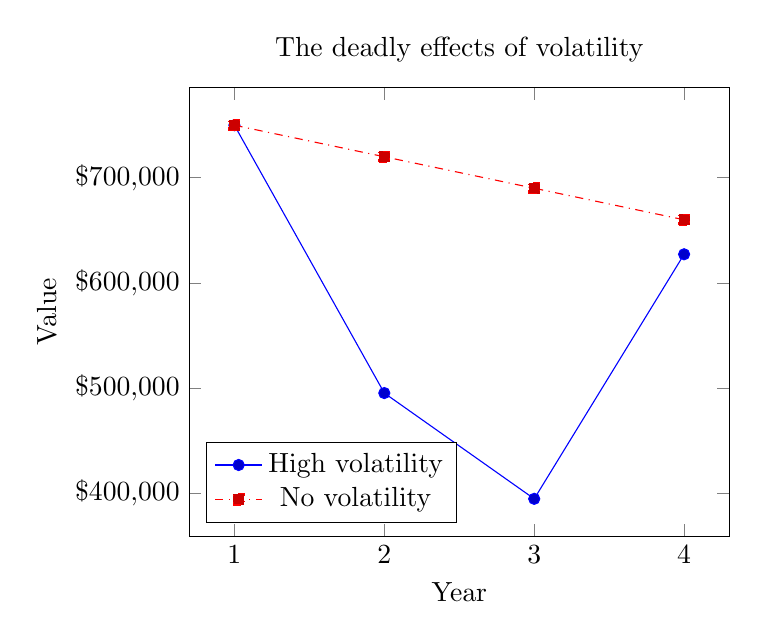
\begin{tikzpicture}
\begin{axis}[
    title=The deadly effects of volatility,
    xlabel={Year},
    ylabel={Value},
    xtick={1,...,4},
    scaled y ticks=false,
    legend pos=south west,
    yticklabel={$\$\pgfmathprintnumber{\tick}$},
    yticklabel style={/pgf/number format/fixed},
]
\addplot+[style={solid}] coordinates {
    (1, 750000)
    (2, 494998)
    (3, 394284)
    (4, 627140)
};
\addplot+[style={dashdotted}] coordinates {
    (1, 750000)
    (2, 720000)
    (3, 690000)
    (4, 660000)
};
\legend{High volatility,No volatility}
\end{axis}
\end{tikzpicture}
\end{figure}

What happened here was that you had to sell more shares in order to reach the same dollar figure of \$30,000. If the stock is selling for \$10 per share, then you only need to sell 3,000 shares to fund your \$30,000 withdrawal, but the year that it dropped to \$6 per share, you were forced to sell 5,000 shares. High volatility has the effect of magnifying your withdrawals.

In this example, the drop happened in the first years of taking withdrawals. It could have also been the reverse, and skyrocketed in the first years, which would have had the opposite effect. If the stock market was booming after you started taking withdrawals, you'd need to spend fewer shares in order to withdraw your \$30,000, thereby increasing your portfolio value. Then, if the same drop happens ten years later, your portfolio would have been much stronger to withstand the same onslaught. So it all depends on timing and volatility.

Volatility risk is one of the greatest investment risks you face when you start taking withdrawals. If you lose a huge portion of your portfolio right off the bat like that, and yet you still need to withdraw money, then your financial future will be in peril.

That's exactly what happened to me.

I retired in February, 2008. The stock market immediately started dropping, and then in October, I faced the greatest stock market crash since The Great Depression. To make matters worse, all of my investments were crashing at the same time, so diversification did nothing to soften the blow. I ended up losing a lot of money. I had some contingency plans, but this was beyond what I could reasonably plan for, so my resolve was really put to the test. All those ``yeah, buts\ldots'' I've heard over the years came to haunt me.

I dropped everything I was doing for six months and focused entirely on the catastrophe. I panicked a few times, then focused, then panicked some more, and focused again. It was scary. First, I looked for even more ways to cut costs that didn't significantly harm my quality of life. Then I pulled out the contingency plans. I had several nice-to-have expenses that I could easily cut in case of emergency. I cut them all, and I was still drowning. I started cutting out some \emph{really}-nice-to-have expenses. Then I started looking for a cheaper place to live.

Meanwhile, I was researching investing again, scouring websites, and reading books. I was trying to figure out how I could have better prevented this disaster and how I can avoid it in the future. Most importantly, I was trying to figure out how to stop the bleeding immediately. Then I did something very naughty: I sold everything.

\emph{Don't try this at home.} If your portfolio is evaporating before your eyes, selling is usually the worst thing you could possibly do. It's the nature of volatility that your investments will recover, and it's the nature of our psychology that our fears will keep us from buying back in before that happens.

However, my choice to sell wasn't out of panic. It was a big risk, and I was perfectly aware of this. It was a decision I made after a lot of thought and research. It was clear that the crash I'd seen so far was only the beginning, but more importantly, I knew this was a unique recession, one never before seen in history. All investment wisdom is based on what we've learned from history. There was no precedent for this. Extreme times called for extreme measures. I may have an investment ``religion,'' but I'm not a fundamentalist. I can still believe in buying and holding index funds, but that doesn't mean that I'm unwilling to make exceptions at the right times, like when I see my entire retirement dream vanishing before my eyes.

The way I figured it, my retirement dream was already gone if I'd let it continue on its present course. Something had to be done. In the worst case, I'd have to go back to work and start over again, and I was already sort of resolved to do this, but at least this way I would go down fighting.

I researched for another few weeks, and then started buying back in, slowly at first, with a whole new portfolio. This new portfolio has several features that I will describe in the next section. I designed it to not only withstand future catastrophes better, but to also take advantage of the current low prices and therefore bring me out even further ahead than when the whole mess started.

The choices I made turned out to be excellent, overall. I was correct that it was only the beginning. It was beneficial to sell when I did and buy back in at lower prices, even though I didn't time it perfectly (no one can). I'd promised myself that I would buy back in \emph{before} it felt safe, so as to avert the risk of not being there for the big recovery. But I did take a huge risk by selling. What if it recovered quickly? I'd have sold at the lowest point, losing a huge opportunity for recovery.

Nonetheless, my plan worked out fabulously. I did indeed end up quite a bit further ahead than when this all started. Only a few years later, I had more money than I had when I first retired, even after inflation. I not only averted the crisis, I used it as an opportunity to position myself even better than when I started.

\section{Investing for growth or income}
As I researched for my new portfolio, I was considering the one disadvantage I had as a retiree: I was taking out regular withdrawals. If this weren't the case, I could have easily weathered the storm and watched everything recover completely. But I knew that even just one or two years of huge losses would be much more severe for me long-term if I took withdrawals in those years.

Like individual stocks, portfolios as a whole also tend to be classified as either \emph{income, growth,} or some combination of both. An income portfolio is one that is designed to give pay-outs at regular intervals, with very little volatility. A growth portfolio is one that is designed to grow over time, with a lot of volatility. This captures the biggest trade-off in investing---risk is usually rewarded with greater growth over time.

I also considered the other unique aspect of my situation: I retired at a young age. That means that I will be holding these investments longer than most retirees, so I have longer to ride out the volatility, even though I will be taking withdrawals along the way. What I needed was a portfolio that was less volatile than pure growth portfolios and more volatile than pure income portfolios, but still provided steady income along the way. What I needed was a combination growth and income portfolio.

As I researched this, one thing that became clear was that I needed more \emph{dividends.} Dividends are regular payments made to shareholders, from the income the companies earn. Dividends do tend to go down during recessions, but not as significantly as the share prices. If I could invest in things that gave more dividends, I figured, and take a larger portion of my withdrawals from those dividends, then I wouldn't need to sell so many shares during recessions. I had avoided dividends before retirement because they are taxed at a higher rate than long-term capital gains, but I'm in a much lower tax bracket now that I'm retired, so avoiding dividends for tax purposes isn't necessary.

Another thing I discovered, or rather, re-discovered, is \emph{costs.} Until then, I hadn't looked as closely at investment costs as I should have. Fees are like the dirty little secret of the mutual fund and brokerage industries. It's in the interest of these industries to avoid talking about them. The only reason they talk about fees to the extent they do is because the Securities Exchange Commission forces them to, and I realized that they still don't tell the half of it.

Despite their low costs, I was running into some limitations of index funds. Like any other mutual funds, index funds are purchased from the mutual fund company itself, each share representing underlying stocks and bonds owned by the fund company. If \emph{you} buy or sell many shares, \emph{they} must buy or sell many shares. This incurs significant costs to the shareholders, so responsible fund companies will institute limits and penalties on how often shareholders may buy and sell their shares.

Another issue with mutual funds, particularly troublesome in volatile times, is that they have up to a one-day delay in their share price, or \emph{NAV.} At the end of each day, they update the NAV, and when you buy, you pay the NAV on the \emph{next} cycle, so you don't know what that NAV will be. That can be risky during times of high volatility.

This was when I discovered \emph{Exchange-Traded Funds,} or \emph{ETFs.} These are a lot like index funds, but they're traded like stocks. You buy them from a stock broker just as you would stocks. There are no limits or penalties on buying or selling shares, since the brokers deal with such large volumes of them, called \emph{creation units.} Since the fund company doesn't have to buy or sell frequently, they tend to be more tax-efficient as well. Since ETFs are handled by stock brokers, rather than the fund companies that offer them, they also have lower trading, management, and marketing costs than even most index funds.

ETFs were initially used by day traders, but their low costs, tax efficiency, and lower volatility risk also made them great candidates for buying and holding. In fact, buying and holding ETFs minimizes their only disadvantage, which is the trading fees. Brokers charge brokerage fees to trade them, just as they do for stocks.

ETFs have their own limitations, however. Due to the brokerage cost of trading them, it's important to find a low-cost brokerage firm. Also, you should only buy ETFs that have a low \emph{average bid/ask spread.} This is the difference between the amount you pay to buy a share and the amount you could sell it for at any given time. It's a hidden cost of trading that must be accounted for. Most ETF companies should be able to tell you the average bid/ask spread of their ETFs.

Something else I did in my new investment strategy was over-invest in stock funds. By the time I bought back in, I had quite a bit more stock exposure than I did before. This caused a bit more volatility during that year as the market struggled to incorporate all the news, but it didn't last very long. First it started to stabilize, then I saw a nice recovery, and a year later, I sold some of them off and bought back into bonds. This allowed me to take advantage of the under-priced stocks.

\section{Buying individual stocks}
Buying and holding a diverse allocation of broad index funds using ETFs is the strategy I use for most of my investing. However, sometimes I use a small portion of my portfolio for more targeted investments. It also serves as a form of diversification, which is what Modern Portfolio Theory requires. Individual stocks and sectors often behave differently than the market as a whole.

When buying individual stocks, the goal is to buy low and sell high. This sounds simple but it's not easy. For one thing, what does ``low'' mean? For most things we buy, we can compare the prices to see which one is cheaper. So it seems intuitive that we could compare the share prices of the investments we want to buy. But a stock price is fairly arbitrary, and depends on how many shares are outstanding.

What you're looking for aren't stocks with a low share price, but stocks with a lower share price than is justified by its value. The same is true for any other kind of bargain-hunting. For example, if you see a car selling for much less than other, similar cars, it might be a bargain---or it might be a lemon. The only way to know the difference is to look under the hood.

There are some ratios you can look at quickly to get a sense for how high or low the price is relative to its assets and its capacity to generate earnings. One such number is the \emph{Price/Earnings ratio,} or \emph{P/E ratio,} which is the stock price divided by the annual earnings, or how much each dollar of annual earnings costs you. This will be lower for investments that have poor future prospects or is not expected to grow much, and higher for investments that are expected to grow. Like any business you buy, you'd pay more for one that is expected to grow quickly.

Another number is the \emph{Price/Book ratio,} which is the stock price divided by the assets owned by the company, or how much each dollar of assets costs you.

Another number is the \emph{Price/Sales ratio,} which is the stock price divided by the annual sales, or how much each dollar of annual sales costs you. Sales are different from earnings. They don't account for the expenses a company has. For example, if a company has a low Price/Sales ratio but a high Price/Earnings ratio, it means that the company is actually really good at earning money, but they're also really good at spending it. Just as you saw in Chapters 1 and 2, both the income and spending components are important. It's often easier to cut costs than it is to get more income, so if you believe the company will do a good job at cutting costs, then this might be a good deal.

After you look at all these numbers, you'll know whether the price is low, but you still won't know why. Just as in the example of shopping for a car: you see the price tag, and you know it's priced low relative to similar cars, but you don't know why. It's up to you as a buyer to closely examine the car and ask the seller questions about it to make sure it's the bargain you hope it is. Likewise, you need to examine an investment, research their balance sheet, income statement, and cash flow statement, read their news, and listen to management conference calls, to determine if it's a bargain. Learning how to do this takes a lot of time, and I'm still a novice myself, but the payoff can be enormous.

Difficult as this may seem, the hardest part of buying low and selling high is actually psychology. Our impulse is to buy high and sell low. When things are going well, we want more of it. When things are going poorly, we want out before it gets worse. It's essential that you be a contrarian. You need to be on a shopping spree when everyone else is talking about the pending apocalypse. You need to be a cynic and start selling off when everyone is talking about how great things are and that it can only get better. This came easy for me because I've always been a bit of a rebel.

When there's a stock market crash, panic ensues. People sell off their investments out of fear. Their fear overpowers their rationality, so they'll sell at any price, even if that price is obviously lower than the company is worth.

During the 2008 crash, some of America's strongest companies were trading at lower than their book value (Price/Book was less than 1). That means that these sellers were saying these companies had no hope of ever turning a profit, that they weren't even worth the property they owned. It was possible that these companies were so worthless that all they could do from now on is lose money, but these were good, solid companies with strong earnings until the big crash. Investors were in such a panic to sell that they were practically giving these companies away. This is an excellent time to snap up some great deals. I bought some shares of a few companies during this time. One of them tripled and another doubled in value in less than a year before I sold it.

\section{Designing your portfolio}
What should your portfolio look like? There are many ways to answer that question. Investing is a personal thing, and depends on many factors specific to you: your age, values, goals, fears, and hopes. I can't tell you exactly what your portfolio should look like, but I can give some general guidelines, and explain the process I used to come up with mine.

I sought out great minds that I trusted. One of these, Warren Buffett, doesn't write very much. However, there were five others that have written good books: Bernard Malkiel, John C. Bogle, William Bernstein, Richard A. Ferri, and Roger Gibson. They each made their own portfolio recommendations, and I used this as a guide. I compared all five recommendations side-by-side and filled in the blanks with educated guesses. I've included two of the five portfolios at the end of this section.

First, decide how you want to divide your portfolio between the two major types of investments: stocks and bonds. This depends on your age and risk tolerance. The more bonds in your portfolio, the less volatile it will be, but also the less it will grow. The younger you are, the longer you have to ride out the storms, so you'll want more stocks because that will give you more growth. If you're older, you'll want more bonds because you don't have the same luxury to ride out the volatility.

Likewise for risk tolerance: if you tend to freak out when there are crashes, you'll want more bonds, but if you know you can keep your cool, you'll want more stocks so you can take advantage of their superior growth. Additionally, once you start taking withdrawals, no matter how old you are, you'll want more bonds because you're much more susceptible to volatility.

Start with an allocation based on your age. If you're under 40, your allocation should be 90\% stocks, 10\% bonds. Starting at age 40, add 3 percentage points of bonds every 2 years. For example, at 40, change your allocation to 87\%/13\%, at 42, change it to 84\%/16\%, etc.

Now adjust for your risk tolerance. If you tend to freak out a little during recessions, add 10 percentage points of bonds. If you tend to freak out a lot, add 10 more. This is your portfolio, so it's entirely your choice how much adjustment you need to make for you to feel comfortable. If you choose something too aggressive for your risk tolerance, and you end up selling out of fear, then that extra little bit of growth you got would do you no good, so if you're not sure, be conservative and lean toward more bonds rather than less.

Once you start taking withdrawals, add another 5 percentage points of bonds, and also consider investing more in dividend-bearing investments.

Next, you must decide how much exposure you'll have to international markets. International investing has historically been important for diversification because they offer relatively low correlations with domestic investments, although that has been changing as our economy becomes more global. Some argue that it's pointless to invest internationally because it's just more risk with little benefit. Others argue that international is the way to go because they believe America will no longer be the economic super power it once was. Most experts believe it's best to have at least some exposure to international investments. How much is up to you. It depends on which experts you agree with and how much you agree with them. I believe 20\% is a good amount of international exposure.

You should now have divided your portfolio into four asset classes. For example, let's say you decided on 60/40 for your stock/bond mix and 80/20 for your domestic/international mix. You just multiply each percentage of stock/bond with a percentage from domestic/international. $60\% \times 80\%$ is 48\% domestic stocks. $60\% \times 20\%$ is 12\% international stocks. $40\% \times 80\%$ is 32\% domestic bonds. $40\% \times 20\%$ is 8\% international bonds.

Now it's time to divide up each of these four asset classes further. For stocks, you have a few different ways you can diversify. One is company size. Large companies perform differently than small companies, so you should have some of both. There are four main size categories: large-cap, mid-cap, small-cap, and micro-cap. Another way to diversify stocks is \emph{growth} versus \emph{value,} which I explained in the Investment Basics section. Both perform roughly the same, but they tend to behave differently, which makes them good candidates for diversification. You should have some of both. You could get them as separate funds, or you could get them both in a \emph{blend fund.}

In international stocks, you have similar distinctions as above, but you can also diversify by region. The main geographical categories are Europe, Pacific Rim, and Emerging Markets. Pacific Rim includes many non-European, first-world countries like Japan, Singapore, and Australia. Emerging Markets includes many of the third world countries. Of the three, Europe is known to behave the most like American stocks and is the least volatile. Emerging Markets behaves the least like American stocks and is the most risky and volatile. Pacific Rim is in the middle, both in correlation and risk. You should probably own some of all three, either separately or together in one fund.

There are non-company stocks you can also buy for additional diversification. A \emph{REIT} is a \emph{Real Estate Investment Trust.} Rather than owning parts of a company, you own parts of corporate real estate. You're paid rent in the form of dividends. You can also buy precious metals and other commodities. Gold is known to be extremely volatile and doesn't perform well long-term, but it may be good to have some in your mix because it tends to have a very low correlation with most other stocks, and is also useful for lowering inflation risk. I don't invest in gold myself.

For bonds, you can diversify based on type, quality, and term. There are government bonds and corporate bonds. Some government bonds worth looking into are \emph{TIPS} and \emph{GNMA.} TIPS is designed to protect you from inflation, which is a good way to lower inflation risk. GNMA is the government mortgage bonds.

The two main categories of quality are \emph{investment grade} and \emph{high yield.} Investment grade bonds are issued by entities with a good credit rating and a history of not defaulting. High yield used to be called \emph{junk bonds} but that name turned people off. High yield bonds are for organizations with poor credit ratings and some history of defaulting, but their rates are much higher to compensate for that risk. So, you can expect the risk and volatility of high yield bonds to be greater than investment-grade bonds, but you can also expect higher long-term growth. For the sake of diversification, it's good to have some of both.

There are short-term, intermediate-term, and long-term bonds. This refers to how long until the loans need to be paid back. The longer the term, the higher the risk, but also the higher the rates. However, long-term bonds don't tend to give enough growth to compensate for its greater risk, so it's better to just stick to short-term and intermediate-term bonds.

International bonds aren't easy to find. As far as I know, there's only one company, DFA, that offers international bond funds that distinguishes between the above three factors, and that company doesn't actually offer these funds to the general public. The amount of international bonds you'll own will probably not be very high anyway, so this doesn't matter much. You can just buy a generic international bond fund. However, there are some good international bond ETFs available to the general public.

How much you divide your portfolio between each of these many types of investments doesn't matter as much as the main two divisions between stocks/bonds and domestic/international. Past this, experts have very different opinions on how portfolios are allocated, but there does tend to be a few common patterns: Growth and value are often divided equally, and it's common to have more large-cap and mid-cap than small-cap and micro-cap, more domestic than international, more Pacific Rim and Europe than Emerging Markets, and more short-term and intermediate-term investment-grade bonds than high yield bonds, TIPS, and GNMA.

\begin{table}[ht]
\caption{Model portfolios}
\label{tab:portfolios}
\centering
\begin{tabular}{l r r r r r r}
\\\hline
\\\hline
& \textbf{Mason} & \textbf{Ferri} & \textbf{Malkiel}\\
\hline
\textbf{\emph{Stocks}} & \textbf{\emph{59.97\%}} & \textbf{\emph{60.00\%}} & \textbf{\emph{65.00\%}}\\
\textbf{U.S. Equity} & \textbf{43.88\%} & \textbf{48.00\%} & \textbf{47.00\%}\\
Large growth & 3.30\% & 15.00\% & 11.50\%\\
Large value & 12.35\% & 15.00\% & 11.50\%\\
Mid-cap growth & 5.63\% & 0.00\% & 0.00\%\\
Small growth & 4.63\% & 0.00\% & 7.00\%\\
Small value & 0.00\% & 9.60\% & 7.00\%\\
Microcap & 2.10\% & 2.40\% & 0.00\%\\
Real estate & 3.80\% & 6.00\% & 10.00\%\\
Speculation & 9.92\% & 0.00\% & 0.00\%\\
\textbf{Intl. Equity} & \textbf{16.09\%} & \textbf{12.00\%} & \textbf{18.00\%}\\
Pacific Rim large & 5.75\% & 3.60\% & 6.00\%\\
Europe large & 1.01\% & 3.60\% & 6.00\%\\
Intl. small cap & 2.81\% & 2.40\% & 0.00\%\\
Intl. value & 1.62\% & 0.00\% & 0.00\%\\
Emerging markets & 4.89\% & 2.40\% & 6.00\%\\
\\
\textbf{\emph{Fixed income}} & \textbf{\emph{40.03\%}} & \textbf{\emph{40.00\%}} & \textbf{\emph{35.00\%}}\\
\textbf{Bonds} & \textbf{34.94\%} & \textbf{38.00\%} & \textbf{30.00\%}\\
Invest. grade & 7.50\% & 7.92\% & 12.50\%\\
High-yield & 4.15\% & 7.92\% & 0.00\%\\
TIPS & 6.97\% & 7.92\% & 5.00\%\\
GNMA & 4.30\% & 0.00\% & 12.50\%\\
Short-term & 8.57\% & 10.29\% & 0.00\%\\
Intl. bonds & 3.34\% & 3.96\% & 0.00\%\\
\textbf{Cash} & \textbf{5.09\%} & \textbf{2.00\%} & \textbf{5.00\%}\\
Money market & 5.09\% & 2.00\% & 5.00\%\\
\hline
\end{tabular}
\end{table}

As an example, Table~\ref{tab:portfolios} at the end of the chapter shows my current portfolio target allocation next to two of the five model portfolios I based it on, from the books \emph{All About Asset Allocation} and \emph{A Random Walk Down Wall Street.} These books didn't spell it out exactly like it is on this table, but I filled in some of the blanks myself in order to compare them side-by-side.

Due to the differences of opinion between the experts, and individual factors such as age, goals, and risk aversion, this is really something you need to customize. I made many choices that disagreed with the experts because I weighed the arguments made in the various books and decided where I stood on those, and whether they applied to me. I favor value and mid-cap companies; I want lots of dividends; I add a small speculative element; and I don't want to invest in oil or gas. Then I tweaked the numbers based on my age, goal, and risk tolerance. I also occasionally tweak this target allocation as things change or as I incorporate new information.

Not only is creating an asset allocation the most personal part of investing, it's also the most important to get right. Most investing experts agree that your asset allocation has far more impact on the performance and risk of your investments than which funds you choose. So, don't spend all your time shopping for funds. Spend more time refining your asset allocation. There are many good books on this subject, some of which are included in the Resources.

\section{Taxes}
Many people are painfully aware of how much payroll taxes they pay, so it's ironic that so few account for it in their investments. This is probably because investment taxes are relatively invisible compared to payroll taxes. They don't show up on their paychecks or monthly statements. But like every recurring, incidental expense, taxes can have a huge impact over time. They are just as important as fees. In a sense, they \emph{are} fees, just paid to a different organization.

Taxes are very political. The major division between each political philosophy is on how this money is collected and spent. Pretty much everyone disagrees with at least one thing the government spends money on, and they don't want to support that with their income. On the other hand, we all use the services the government provides. Some resent it, while others are grateful for those services and are glad to support them.

Taxes should be fair, and it's up to our elected officials to create a fair tax system. They will offer credits, deductions, and adjustments to incentivize certain things and allow for exceptions to the basic tax rules. Your job as an investor is to learn about which of these are relevant for you and take advantage of them. In other words, your goal is to minimize the taxes you're required to pay. This is an easy sell for those who resent taxes, but even if you want to support the system with your taxes, you should still take advantage of all the tax incentives offered to you because that's an important part of the system.

The most fundamental aspect of our tax system is that it is based on earning and spending money. Income tax is for the money you earn, and sales tax and property tax is for the money you spend. Financial independence involves minimizing the amount of money you spend in order to minimize the money you earn. Therefore, by the very nature of the tax system, the closer you get to financial independence, the less you'll be required to pay in taxes. You'll be spending less, so you'll be paying less sales tax. Your food and drug costs will be a larger portion of your total spending, which are not taxed at all. You'll also be earning less, so you'll pay less in income taxes, at a lower tax bracket. More of your income will come from long-term investments, which is taxed at a lower rate than salary.

Interest and dividends are taxed at your normal tax rate. There are also \emph{capital gains,} which are the gains you get from selling an investment at a higher price than you paid for it. The IRS distinguishes between two holding periods. \emph{Short-term capital gains} are gains you made on investments that you held for one year or less. These are also taxed at your normal tax rate. However, \emph{long-term capital gains}, for investments you held for more than one year, are taxed at much lower rates. If your tax bracket is 25\% or higher, you only pay 15\% for your long-term capital gains, which is nearly half of what you'd normally pay. If your tax bracket is 10\% or 15\%, you pay zero taxes on your long-term capital gains.

It's possible to keep your income so low that you pay zero taxes on your long-term capital gains. Take a look at your current tax schedule to see what income this means for you. You will also want to minimize your short-term capital gains. That means only selling your investments if you've held them for at least a year. If you re-balance your portfolio no more frequently than one year and one day, then this should be taken care of for you.

You should also minimize interest and dividends, since these are taxed at your normal rates. This is especially important while you're earning a lot and saving for financial independence, since you'll be in a higher tax bracket. There are a few ways to minimize dividends. One is to invest inside of a tax shelter, which I will talk about shortly. Another way is to use \emph{tax-managed funds.} Another way is to focus on growth funds more than value funds. Once you go into a lower tax bracket, however, it's not quite as important to minimize dividends. I have found that the added advantage of a more stable income outweighs the need to minimize dividends for tax purposes once I achieved financial independence and started taking regular withdrawals.

You should also minimize the \emph{turnover} in any funds outside of tax shelters. Turnover is the percentage of the holdings in a fund that are bought and sold each year. You're not only taxed on the capital gains that you get from buying and selling the fund as a whole, but also from the buying and selling that happens \emph{within the fund} throughout the year. These taxes can really add up fast for high-turnover funds. Look for funds with less than 50\% annual turnover. Index funds are, by their nature, extremely low-turnover funds. Avoid high-turnover funds or put them in a tax shelter.

\emph{Tax shelters} protect your investments from taxes, mainly for retirement purposes. One tax shelter is the 401(k) and 403(b) retirement plans (named after the section of the tax code that created them). You get these through an employer. They deduct a certain amount from your paychecks. Many of them also \emph{match} your contributions, which means that they will pay some amount to your retirement plan for each amount that you pay. You will not be taxed on this or its growth until you retire. I recommend that you take advantage of this matching feature as much as you can, up to the limit. Once you leave your job, you may \emph{roll over} (which is just a fancy way of saying ``moving'') your money from your 401(k) or 403(b) plans into an IRA or Roth IRA.

An \emph{Individual Retirement Account,} also called an \emph{IRA} or \emph{traditional IRA,} does not depend on your job. IRAs provide the same benefits as an employer-sponsored plan with more flexibility but lower contribution limits. Unlike an employer-sponsored plan, you can invest your IRA in anything you want---stocks, bonds, savings accounts, CDs, etc. The IRA itself is just a tax mechanism. Whichever investment vehicle you choose, the IRA only means that you don't have to pay taxes on what you contribute or on its growth until you withdraw it.

For the 401(k), 403(b), and IRA, you will be taxed when you take withdrawals. This is called \emph{tax deferral.} This is very much to your advantage because your earnings will have grown tax-free for all those years, and you will probably be in a lower tax bracket when you start taking withdrawals.

A \emph{Roth IRA} is very similar to an IRA, but is the opposite from traditional IRAs in one significant way. In an IRA, you're not taxed on what goes in, but on what comes out. In a Roth IRA, you're taxed on what goes in, but not on what comes out.

Whether you would be better off contributing to an IRA or Roth IRA depends on your tax bracket. If you're in a high tax bracket, you'd be better off contributing to an IRA because you won't be taxed until you're in a lower tax bracket later. You can also later convert an IRA to a Roth IRA and get taxed right away if you go into a lower tax bracket.

However, Roth IRAs are better than IRAs for most people. It's usually better to pay taxes right away and not pay any taxes on its growth, because over time, the growth of investments tends to far overshadow the original contributions. Another advantage of the Roth IRA is that you can withdraw the original contributions any time you want,\footnote{The one exception is that you must wait 5 years before doing so for any money you've converted from a traditional IRA to a Roth IRA.} so the Roth IRA can also serve as a supplemental emergency fund.

Another tax shelter is a \emph{Health Savings Account} or \emph{HSA.} There are health insurance plans that incorporate these. You put money into this account tax-free, which can grow over time. When you get sick, you can withdraw the money tax-free. This is an excellent option for people who are relatively healthy, due to their extremely low monthly premiums and tax savings.

There are also tax shelters for saving for education, but most tax shelters are designed for retirement.

The government has a very specific idea of what retirement means. On the surface, their definitions may seem to differ from those who want financial independence in the form of early retirement. The standard rule is that you can't retire until you're $59 \frac{1}{2}$ years old. However, they provide a little known exception to this rule for early retirees: you may withdraw your money from your IRA or Roth IRA at regular intervals, on a schedule according to your life expectancy. This is called the \emph{72(t) exception.} All the IRS cares about is that you're actually retired, and not just taking money out whenever you feel like it. Therefore, once you start taking withdrawals on a schedule, you must continue doing so indefinitely.

You might not even need to use 72(t). If you're investing a lot of money very quickly, you will hit your tax shelter contribution limits, so you will also be investing money outside of your tax shelter. Once you start taking withdrawals, start with money outside of your tax shelter, and once you've depleted that, then start taking regular withdrawals from your IRA or Roth IRA. Once you've started taking withdrawals from a Roth IRA, you will be able to withdraw all your original contributions tax-free, and will only need to use the 72(t) schedule once you've depleted that.

I actually pay \emph{zero taxes,} legally and with no loopholes. First, I invested heavily in my 401(k), paying zero taxes going in. Once I became financially independent, I rolled over everything into an IRA. After the crash, when I sold everything and bought a whole new portfolio, I reported huge losses that will take me years to recapture. This way, I have zero income for tax purposes, except for the year I sell my home. I would have negative income, if that were possible.

Between this negative income and deductions, I have some wiggle room to move money from my IRA to Roth IRA each year, tax free. Once it's all in my Roth IRA, I can withdraw all of my money tax-free. My expenses are so low that my income will be in the 10\% or 15\% tax bracket, which means that all long-term capital gains from anything not in the IRA or Roth IRA will also be tax-free.

Homeownership also has its perks. Many of the biggest costs for homeowners are deductible from taxes. Mortgage interest and property taxes are entirely tax deductible. Plus, any gains you get from selling it for more than you bought it are also tax-free (up to a limit). You get even more benefit if you rent out some rooms in your home, because this allows you to deduct a portion of your maintenence and repair expenses as well.

In summary, the best way to minimize the tax you're required to pay is to earn and spend as little as possible, use tax shelters, own and live in a rental home, use tax-managed funds outside of your tax shelters, and keep high dividend and high turnover funds in your tax shelters. Maximize your contributions to your 401(k) or 403(b) first, then maximize your contributions to your IRA or Roth IRA, and then invest normally. IRA is tax-free going in and taxed coming out, while Roth IRA is taxed going in and tax-free coming out. It's better to use a Roth IRA unless you're in a higher tax bracket. It's possible to pay zero taxes if you keep your income low enough and you slowly convert your IRA to a Roth IRA over time, with enough deductions or capital losses to capture those conversions.

\newpage
\section{Resources}
\begin{itemize}
\item \textbf{\emph{A Random Walk Down Wall Street,} by Burton Malkiel.} This is the best investing book I've read. I consider it essential reading. It explains everything you need to know about investing, in the most down-to-earth fashion I've ever seen, but without dumbing it down. It demonstrates the Random Walk theory of investing. It is a little long-winded, but it's worth it.

\item \textbf{\emph{Common Sense on Mutual Funds} by John C. Bogle.} If you can only read one investing book, read \emph{A Random Walk,} but if you can read two, read \emph{Common Sense.} When you read this book, you'll understand just how vital it is to minimize investment costs. Although this book is a little dry at times, the way Bogle exposes the evils of the mutual fund industry is amazing.

\item \textbf{\emph{All About Asset Allocation} by Richard A. Ferri.} If you can only read two investing books, read \emph{A Random Walk} and \emph{Common Sense,} but if you can read three, read \emph{All About Asset Allocation.} Other books explain how investing works, but fall short when it comes to the nuts-and-bolts of putting together an actual portfolio. This book assumes you know how investing works, and just explains how asset allocation works and how to put together a good portfolio.

\item \textbf{\emph{Value Investing For Dummies} by Peter J. Sander and Janet Haley.} Don't let the title fool you. Although it's very accessible for the layman, it's also very thorough and detailed. I've read several books on value investing, and this is the best. If you want to learn how to determine if a stock is worth the price, this book will teach you.

\item \textbf{\url{https://advisors.vanguard.com/}} -- The website for Vanguard financial advisors.

\item \textbf{\url{https://personal.vanguard.com/us/funds/tools/recommendation}} -- Vanguard's balanced fund recommendation engine. Answer a few questions, such as risk tolerance and time horizon, and it will recommend a balanced fund intended to meet your needs.
\end{itemize}
